\documentclass[a4paper,12pt]{book}
%\documentclass[a4paper,12pt,landscape,twocolumn,final draft]{book}

%%%%%%%%%%%%%%%%%%%

\usepackage[english]{babel}
\usepackage{blindtext}
\usepackage[a4paper, inner=1.5cm, outer=3cm, top=2cm, bottom=3cm, bindingoffset=1cm]{geometry}
\usepackage[onehalfspacing]{setspace}

%\usepackage{fancyhdr}
\usepackage{graphicx}
\usepackage{titling}


\usepackage[table]{xcolor}
\usepackage{sidecap}
\usepackage{longtable}
\usepackage{helvet}
\usepackage{stackengine}
\usepackage{array,ragged2e}
\usepackage{tabto}
\usepackage{color}

%%%%%%%%%%%%%%%%%%%

%\pagestyle{empty}


\pretitle{%
  \begin{center}
  \LARGE
  
\includegraphics[width=5cm]{debianlogo2.png}\\[\bigskipamount]
%\includegraphics[width=6cm,height=2cm]{logo}\\[\bigskipamount]
}
\posttitle{\end{center}}


\begin{document}

%{\centering
%	\huge \bfseries Debian 7 : Installation steps \\
%	\Large \normalfont written by Bernard Mirguet \\
%	\normalsize \today
%}

%\begin{figure}
%	%\centering
%	\includegraphics[width= 0.7\textwidth]{debian-logo.png}
%	\caption{Menu list}
%\end{figure}


\title{version 7: Be/Fr Installation steps}
\author{bernard.mirguet@gmail.com \\www.nakalogic.com}
\date{March 30, 2015\\\LaTeX} 
\maketitle

%%%%%%%%%%%%%%%%%%%
\tableofcontents

%\fancyhf{}
%\fancyhead[LE]{\leftmark}
%\fancyhead[RO]{\nouppercase{\rightmark}}
%\fancyfoot[LE,RO]{\thepage}
%\pagestyle{fancy}

\chapter[Intro]{Introduction}
\section{Welcome}
Welcome to the step by step Linux Debian 7 installation.

This little sheet of paper just aims to help you to follow the differents screens of an installation. You will learn some basic stuff to know about disk management, partitionning, file systems, ...

%talk about school.

%\section[Filler text]{Purpose}
%\blindtext[10]
%More dummy text\footnote{Et ta soeur?} will follow\footnote{Elle bat lbeure !}.

\section{Informations}
This install is in CLI (Command Line Interface), the second option is to use the GUI (Graphic User Interface). All frames and options are the same. 
\\For the CLI install, the keyboard's keys are: [ENTER = select], [SPACE = option select], [TAB = navigate], [SHIFT TAB = navigate], [ARROW keys = navigate].

\chapter{VirtualBox configuration}
\section{Settings pre-configuration}
\begin{center} \newcolumntype{M}[1]{>{\arraybackslash}p{#1}} \begin{longtable}{M{12cm}|M{4cm}}
\belowbaseline[0pt-\heightof{X}]{ 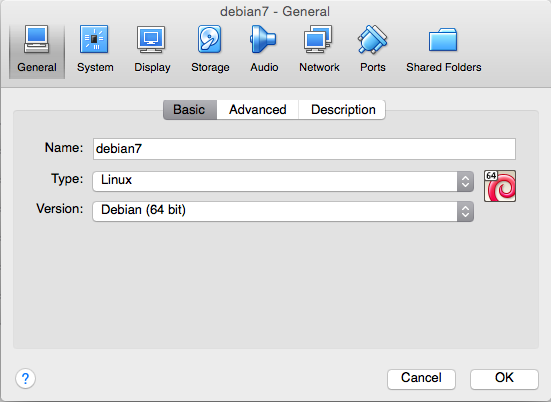
\includegraphics[width=0.7\textwidth]{img/debian7-65.png} } 
& \vspace{0pt} Select your virtual machine and click on "Settings" , "General" tab: enter the vms name 
\end{longtable}
\end{center}
\begin{center} \newcolumntype{M}[1]{>{\arraybackslash}p{#1}} \begin{longtable}{M{12cm}|M{4cm}}
\belowbaseline[0pt-\heightof{X}]{ 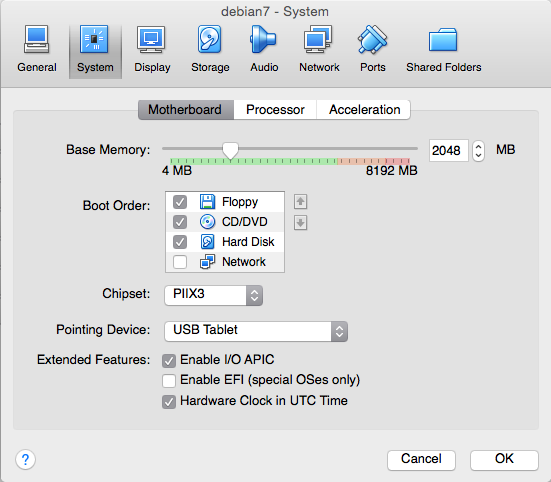
\includegraphics[width=0.7\textwidth]{img/debian7-66.png} } 
& \vspace{0pt} "System" tab: I've got 8 Go RAM, 2048 Mo for install is far enought, minimum for a fast install could be 1024 Mo 
\end{longtable}
\end{center}
\begin{center} \newcolumntype{M}[1]{>{\arraybackslash}p{#1}} \begin{longtable}{M{12cm}|M{4cm}}
\belowbaseline[0pt-\heightof{X}]{ 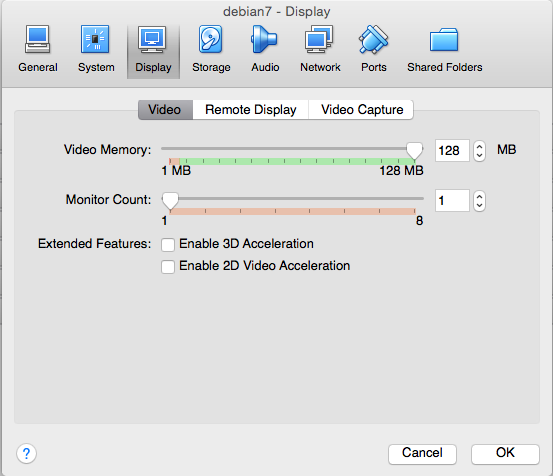
\includegraphics[width=0.7\textwidth]{img/debian7-67.png} } 
& \vspace{0pt} "Display" tab: If you want to install a GUI (Graphical User Interface), slide until 128 Mo of video's memory 
\end{longtable}
\end{center}
\begin{center} \newcolumntype{M}[1]{>{\arraybackslash}p{#1}} \begin{longtable}{M{12cm}|M{4cm}}
\belowbaseline[0pt-\heightof{X}]{ 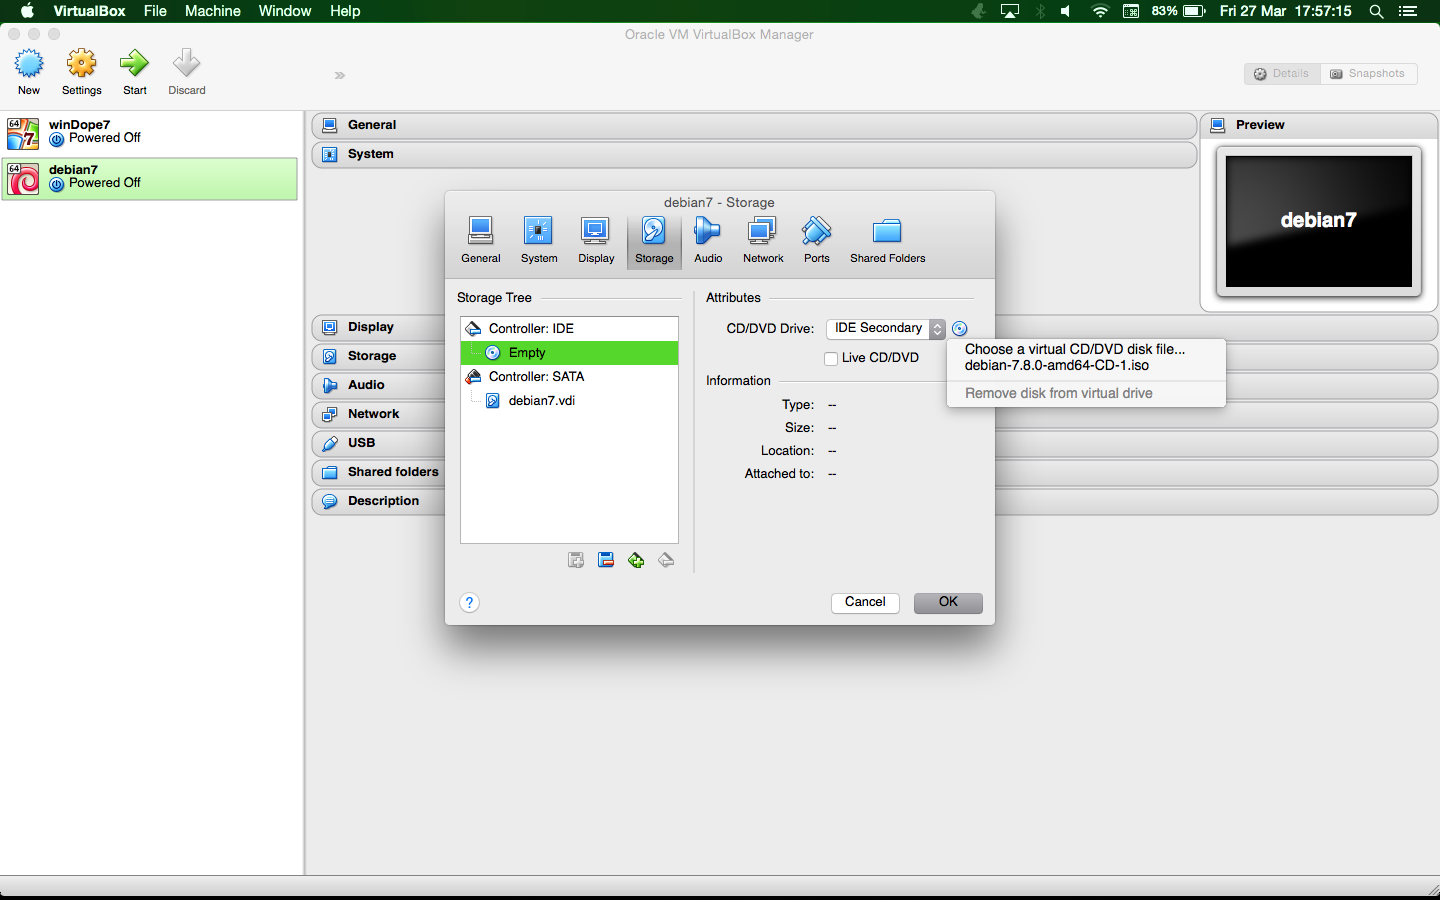
\includegraphics[width=0.7\textwidth]{img/debian7-69.png} } 
& \vspace{0pt} "Storage" tab: Load your ISO disk 
\end{longtable}
\end{center}
\begin{center} \newcolumntype{M}[1]{>{\arraybackslash}p{#1}} \begin{longtable}{M{12cm}|M{4cm}}
\belowbaseline[0pt-\heightof{X}]{ 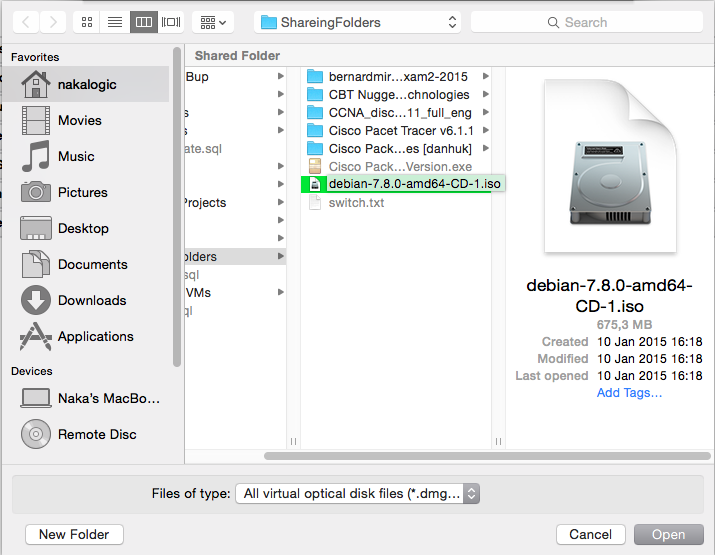
\includegraphics[width=0.7\textwidth]{img/debian7-71.png} } 
& \vspace{0pt} Select your .iso file 
\end{longtable}
\end{center}
\begin{center} \newcolumntype{M}[1]{>{\arraybackslash}p{#1}} \begin{longtable}{M{12cm}|M{4cm}}
\belowbaseline[0pt-\heightof{X}]{ 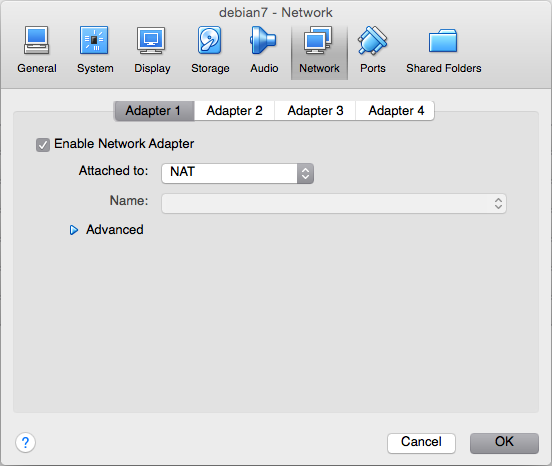
\includegraphics[width=0.7\textwidth]{img/debian7-72.png} } 
& \vspace{0pt} "Network" tab: you can choose NAT (Network Address Translation, your vm will have an internal IP, from the VirtualBox' switch), or "Bridged adapter" (your vm will have an IP from your DHCP (LAN) 
\end{longtable}
\end{center}

\chapter{Steps list}
\section{List}
Here's the full list of operations to follow for your fully (with GUI, Graphic User Interface) Linux Operating System.

\begin{center}
	\newcolumntype{M}[1]{>{\arraybackslash}p{#1}}
 	\begin{longtable}{M{12cm}|M{4cm}}
 		\belowbaseline[0pt-\heightof{X}]{%
   			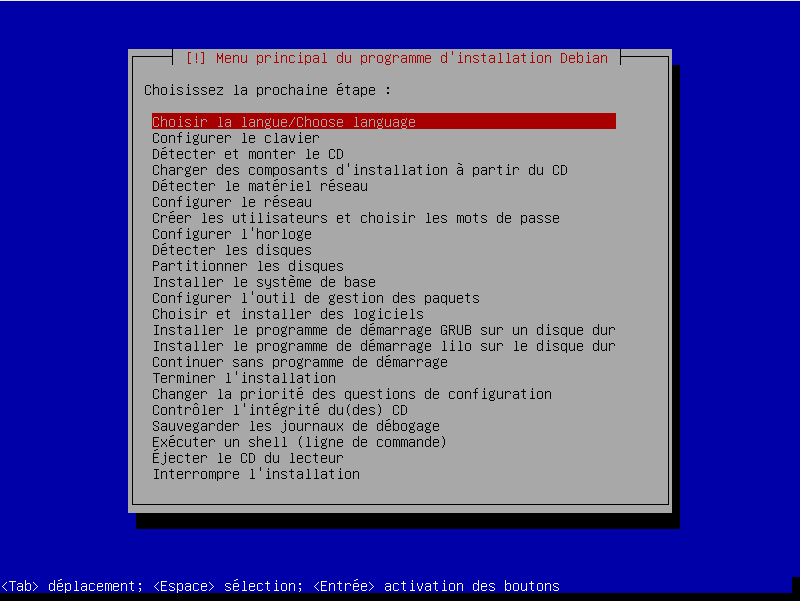
\includegraphics[width=0.7\textwidth]{img/debian7-01.png}%
 		} &
 	\vspace{0pt} Fast description follow 

	\end{longtable}
\end{center}
\pagebreak
% dot listed
%\newcommand{\tab}[1]{\hspace{.2\textwidth}\rlap{#1}}
\begin{itemize}
  	\item Choisir la langue \\ {\color{blue} Francais :)}
	\item Configurer le clavier \\ {\color{blue} Francais / Belge}
	\item Detecter et monter le CD \\ {\color{blue} Automatic}
	\item Charger des composants a partir du CD \\ {\color{blue} Automatic}
	\item Detecter le materiel reseau \\ {\color{blue} Automatic}
	\item Configurer le reseau \\ {\color{blue} Hostname, DHCP}
	\item Creer les utilisateurs et choisir les mots de passe \\ {\color{blue} root password \& user password}
	\item Configurer l'horloge \\ {\color{blue} UTP server}
	\item Detecter les disques \\ {\color{blue} Local disk}
	\item Partitionner les disques \\ {\color{blue} Partitionning theory}
	\item Installer le systeme de base \\ {\color{blue} Automatic}
	\item Configurer l'outil de gestion des paquets \\ {\color{blue} apt source.list, cd, net links}
	\item Choisir et installer des logiciels \\ {\color{blue} GUI, laptop, base}
	\item Installer GRUB sur le disque \\ {\color{blue} Bootloader theory}
	\item Installer LILO sur le disque \\ {\color{blue} none, or choose this bootloader}
	\item Continuer sans programme de demarrage \\ {\color{blue} ... I don't think you really want to do that}
	\item Terminer l'installation \\ {\color{blue} Congratitulation !}
	\item \ldots
	\item Interrompre l'installation \\ {\color{blue} some errors, need to restart install ?}
\end{itemize}



\chapter{Detailed frames}

\section{Choisir la langue}
\begin{center} \newcolumntype{M}[1]{>{\arraybackslash}p{#1}} \begin{longtable}{M{12cm}|M{4cm}}
\belowbaseline[0pt-\heightof{X}]{ 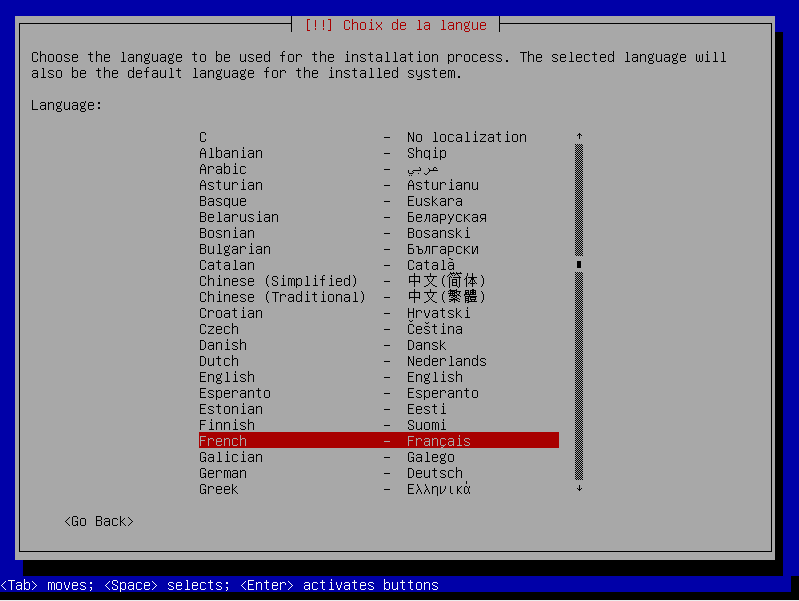
\includegraphics[width=0.7\textwidth]{img/debian7-02.png} } 
& \vspace{0pt} Choose French 
\end{longtable}
\end{center}
\pagebreak


\section{Configurer le clavier}
\begin{center} \newcolumntype{M}[1]{>{\arraybackslash}p{#1}} \begin{longtable}{M{12cm}|M{4cm}}
\belowbaseline[0pt-\heightof{X}]{ 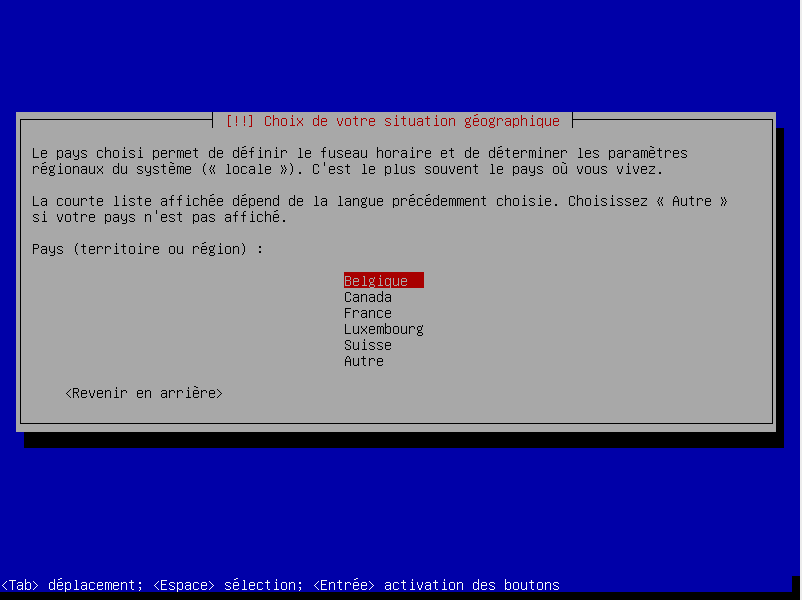
\includegraphics[width=0.7\textwidth]{img/debian7-03.png} } 
& \vspace{0pt} Belgian keyboard
\end{longtable}
\end{center}

\section{Detecter et monter le CD}
Automatic

\section{Charger des composants a partir du CD}
Automatic
\pagebreak

\section{Detecter le materiel reseau}
\begin{center} \newcolumntype{M}[1]{>{\arraybackslash}p{#1}} \begin{longtable}{M{12cm}|M{4cm}}
\belowbaseline[0pt-\heightof{X}]{ 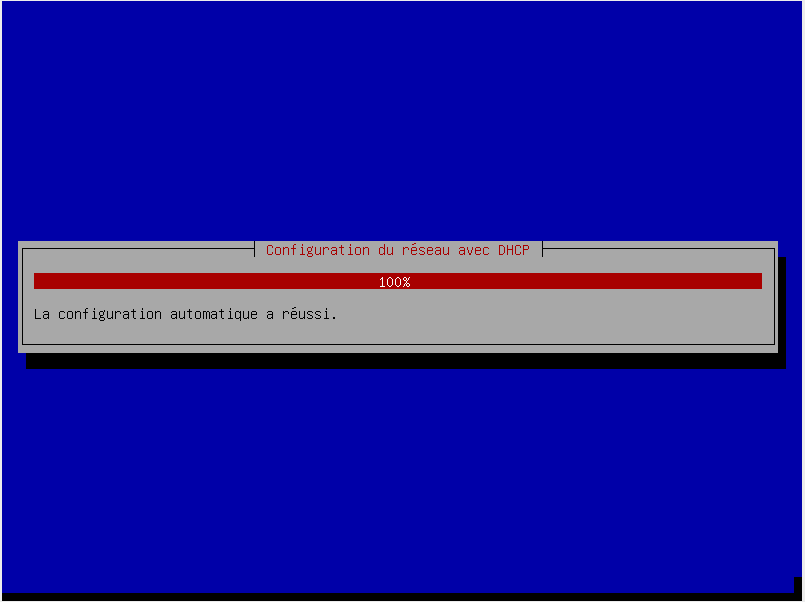
\includegraphics[width=0.7\textwidth]{img/debian7-04.png} } 
& \vspace{0pt} The easiest way is DHCP configuration, for a fixed IP, search on google: linux debian fixed ip /etc/network/interfaces 
\end{longtable}
\end{center}

\section{Configurer le reseau}
\begin{center} \newcolumntype{M}[1]{>{\arraybackslash}p{#1}} \begin{longtable}{M{12cm}|M{4cm}}
\belowbaseline[0pt-\heightof{X}]{ 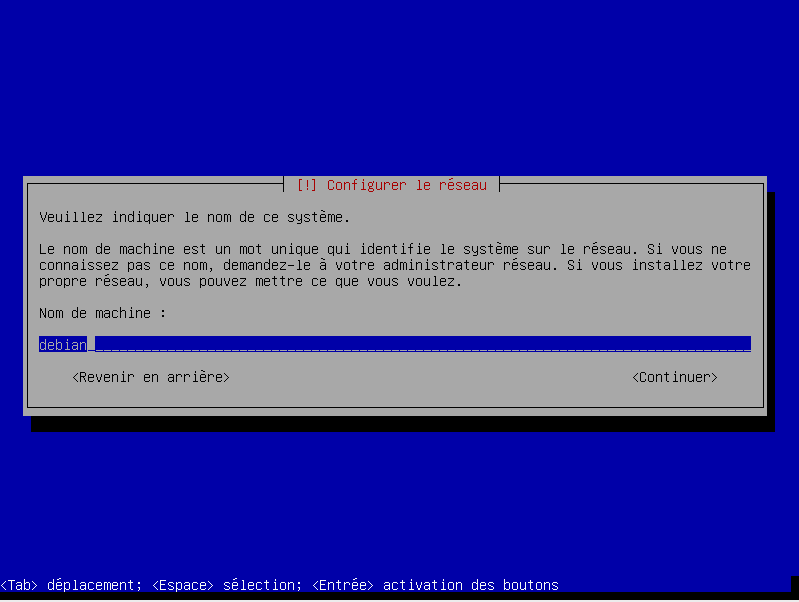
\includegraphics[width=0.7\textwidth]{img/debian7-05.png} } 
& \vspace{0pt} Server's name 
\end{longtable}
\end{center}
\begin{center} \newcolumntype{M}[1]{>{\arraybackslash}p{#1}} \begin{longtable}{M{12cm}|M{4cm}}
\belowbaseline[0pt-\heightof{X}]{ 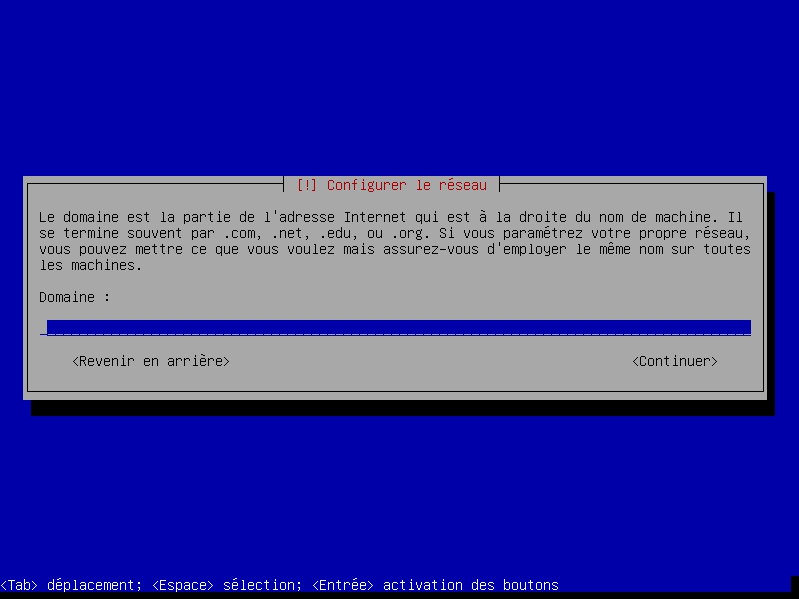
\includegraphics[width=0.7\textwidth]{img/debian7-06.png} } 
& \vspace{0pt} If your local netword is not in a specific domain, leave it empty
\end{longtable}
\end{center}

\section{Creer les utilisateurs et choisir les mots de passe}

\begin{center} \newcolumntype{M}[1]{>{\arraybackslash}p{#1}} \begin{longtable}{M{12cm}|M{4cm}}
\belowbaseline[0pt-\heightof{X}]{ 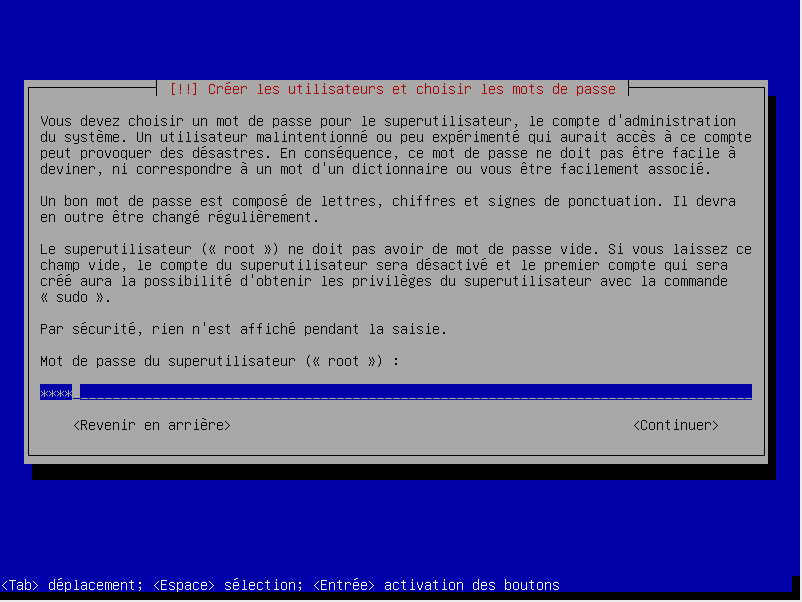
\includegraphics[width=0.7\textwidth]{img/debian7-08.png} } 
& \vspace{0pt} Enter root's password 
\end{longtable}
\end{center}
\begin{center} \newcolumntype{M}[1]{>{\arraybackslash}p{#1}} \begin{longtable}{M{12cm}|M{4cm}}
\belowbaseline[0pt-\heightof{X}]{ 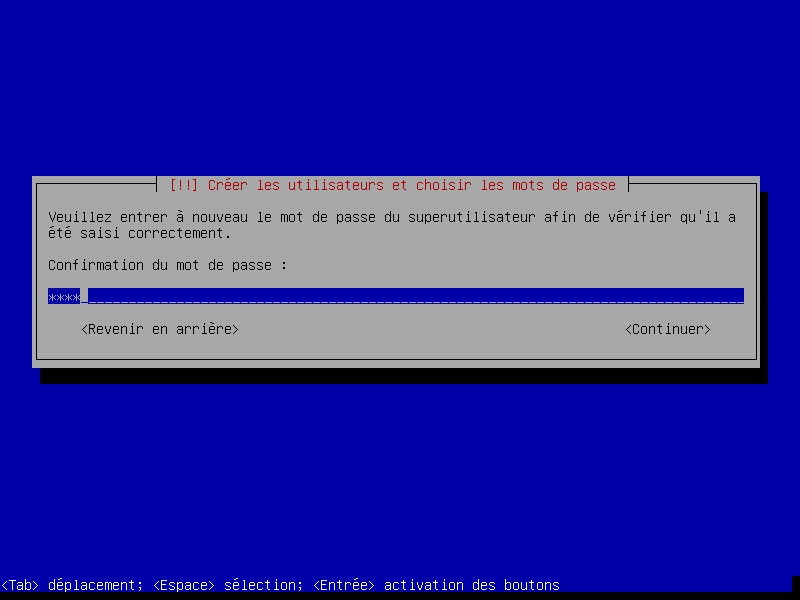
\includegraphics[width=0.7\textwidth]{img/debian7-12.png} } 
& \vspace{0pt} Repeat and confirm the password 
\end{longtable}
\end{center}
\begin{center} \newcolumntype{M}[1]{>{\arraybackslash}p{#1}} \begin{longtable}{M{12cm}|M{4cm}}
\belowbaseline[0pt-\heightof{X}]{ 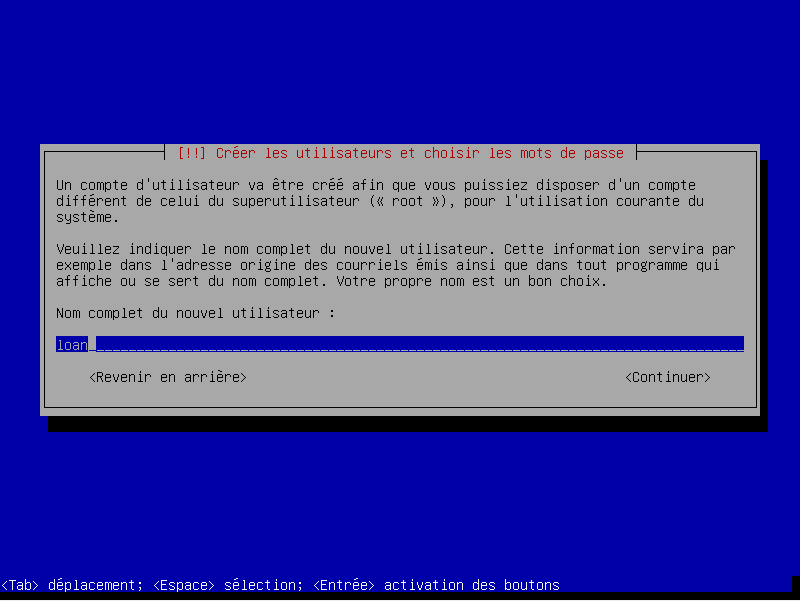
\includegraphics[width=0.7\textwidth]{img/debian7-13.png} } 
& \vspace{0pt} Enter the username of the first new user 
\end{longtable}
\end{center}
\begin{center} \newcolumntype{M}[1]{>{\arraybackslash}p{#1}} \begin{longtable}{M{12cm}|M{4cm}}
\belowbaseline[0pt-\heightof{X}]{ 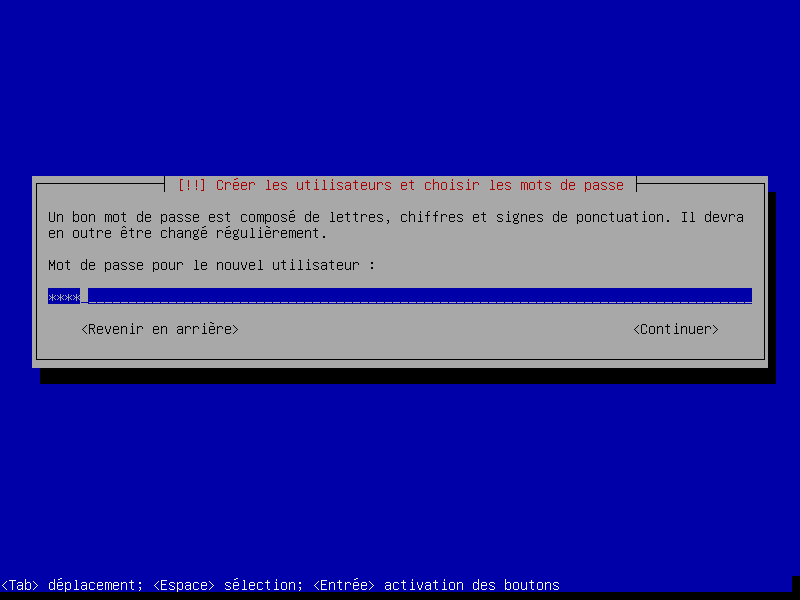
\includegraphics[width=0.7\textwidth]{img/debian7-15.png} } 
& \vspace{0pt} Enter his password 
\end{longtable}
\end{center}
\begin{center} \newcolumntype{M}[1]{>{\arraybackslash}p{#1}} \begin{longtable}{M{12cm}|M{4cm}}
\belowbaseline[0pt-\heightof{X}]{ 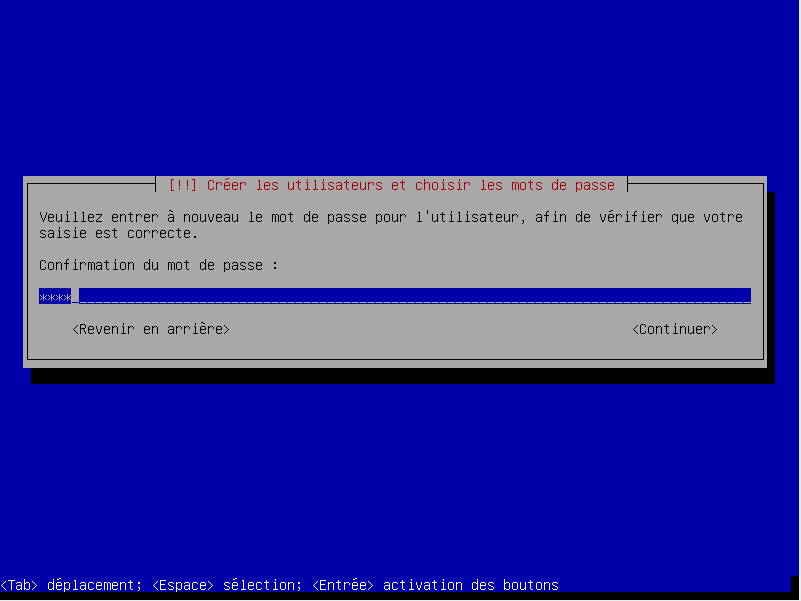
\includegraphics[width=0.7\textwidth]{img/debian7-16.png} } 
& \vspace{0pt} Repeat and confirm the password 
\end{longtable}
\end{center}
\pagebreak


\section{Configurer l'horloge}
Automatic with an UTP server

\section{Detecter les disques}
Automatic

\section{Partitionner les disques}
\begin{center} \newcolumntype{M}[1]{>{\arraybackslash}p{#1}} \begin{longtable}{M{12cm}|M{4cm}}
\belowbaseline[0pt-\heightof{X}]{ 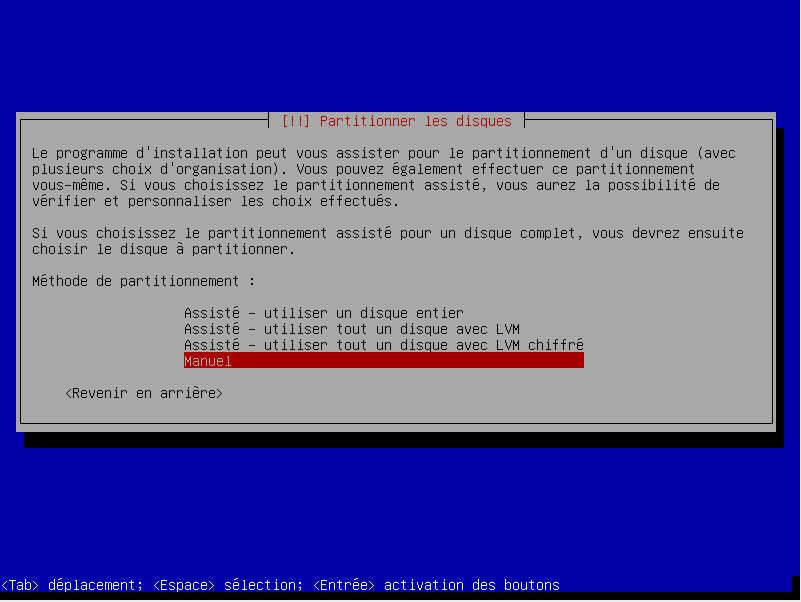
\includegraphics[width=0.7\textwidth]{img/debian7-18.png} } 
& \vspace{0pt} Select "manual" partitionning 
\end{longtable}
\end{center}
\begin{center} \newcolumntype{M}[1]{>{\arraybackslash}p{#1}} \begin{longtable}{M{12cm}|M{4cm}}
\belowbaseline[0pt-\heightof{X}]{ 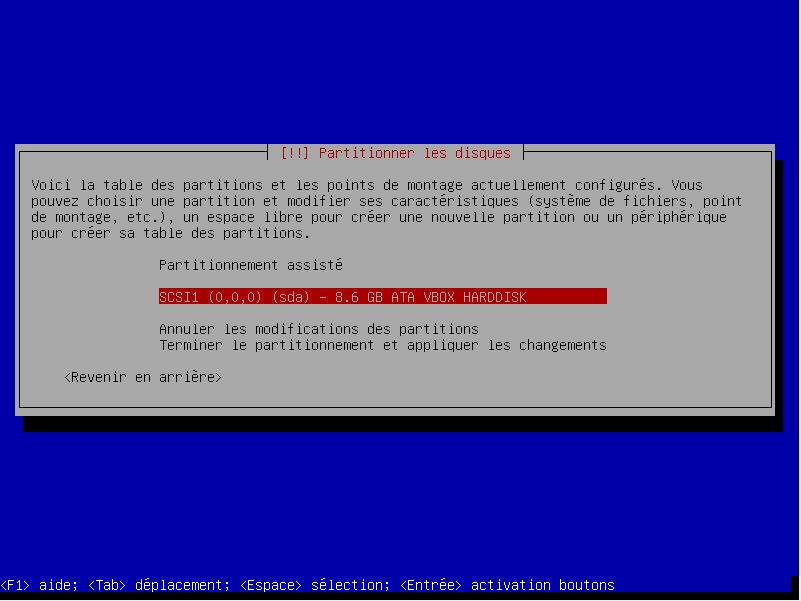
\includegraphics[width=0.7\textwidth]{img/debian7-19.png} } 
& \vspace{0pt} Select the disk, here there's only 1 hard drive 
\end{longtable}
\end{center}
\begin{center} \newcolumntype{M}[1]{>{\arraybackslash}p{#1}} \begin{longtable}{M{12cm}|M{4cm}}
\belowbaseline[0pt-\heightof{X}]{ 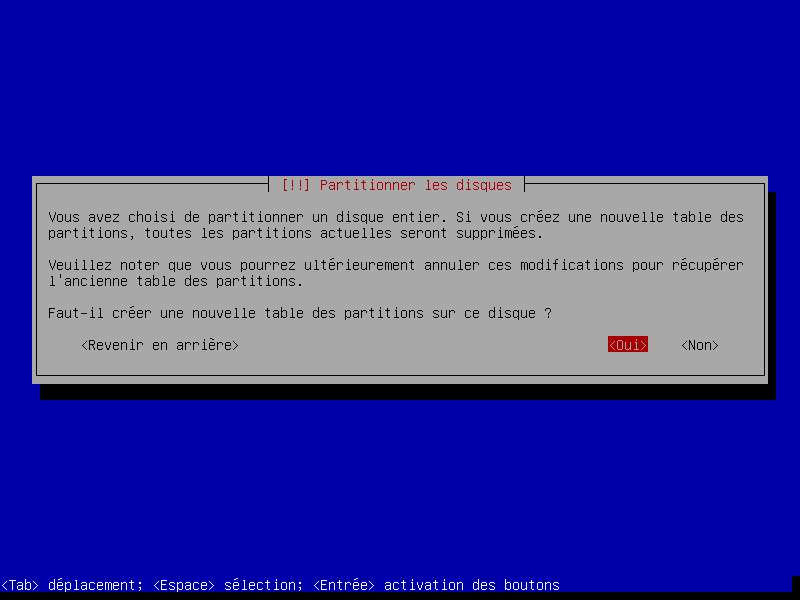
\includegraphics[width=0.7\textwidth]{img/debian7-20.png} } 
& \vspace{0pt} Yes, you want to create a partition table 
\end{longtable}
\end{center}
\begin{center} \newcolumntype{M}[1]{>{\arraybackslash}p{#1}} \begin{longtable}{M{12cm}|M{4cm}}
\belowbaseline[0pt-\heightof{X}]{ 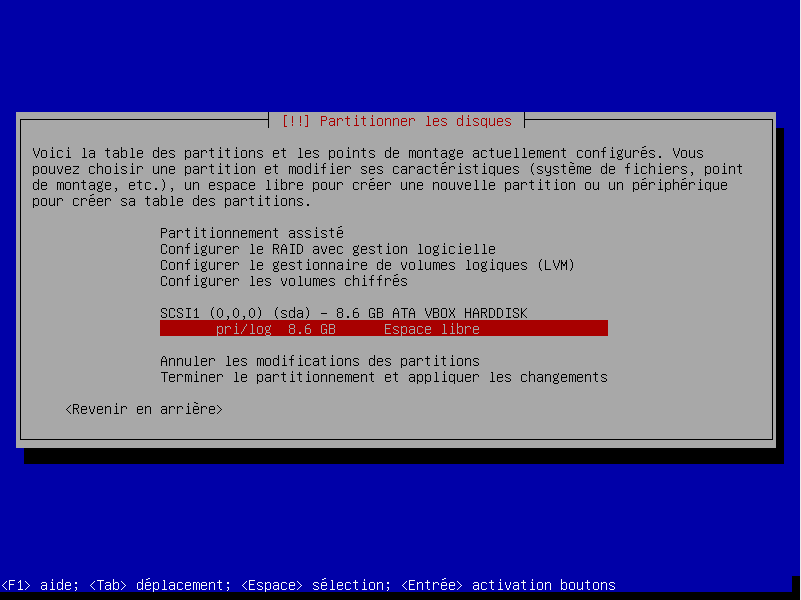
\includegraphics[width=0.7\textwidth]{img/debian7-21.png} } 
& \vspace{0pt} Enter into the new partition 
\end{longtable}
\end{center}
\begin{center} \newcolumntype{M}[1]{>{\arraybackslash}p{#1}} \begin{longtable}{M{12cm}|M{4cm}}
\belowbaseline[0pt-\heightof{X}]{ 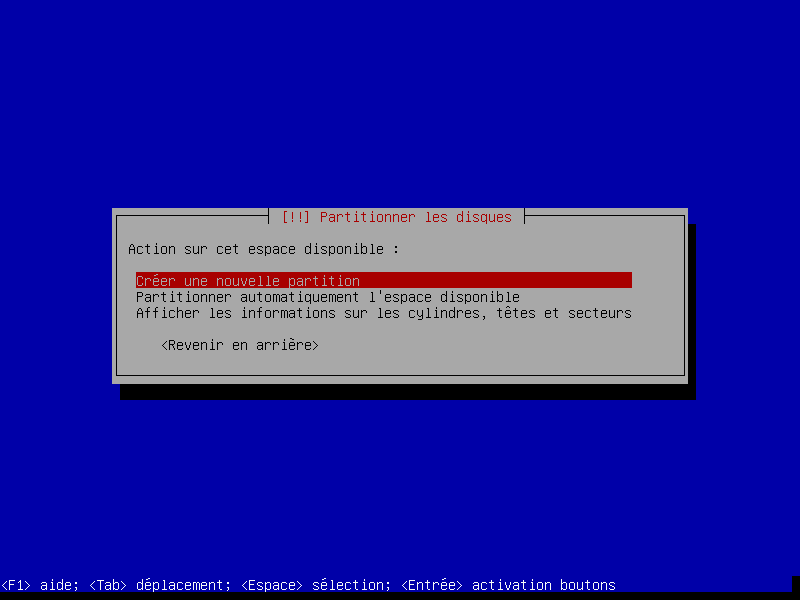
\includegraphics[width=0.7\textwidth]{img/debian7-22.png} } 
& \vspace{0pt} Of course create a new partition (this one is the SWAP)
\end{longtable}
\end{center}
\begin{center} \newcolumntype{M}[1]{>{\arraybackslash}p{#1}} \begin{longtable}{M{12cm}|M{4cm}}
\belowbaseline[0pt-\heightof{X}]{ 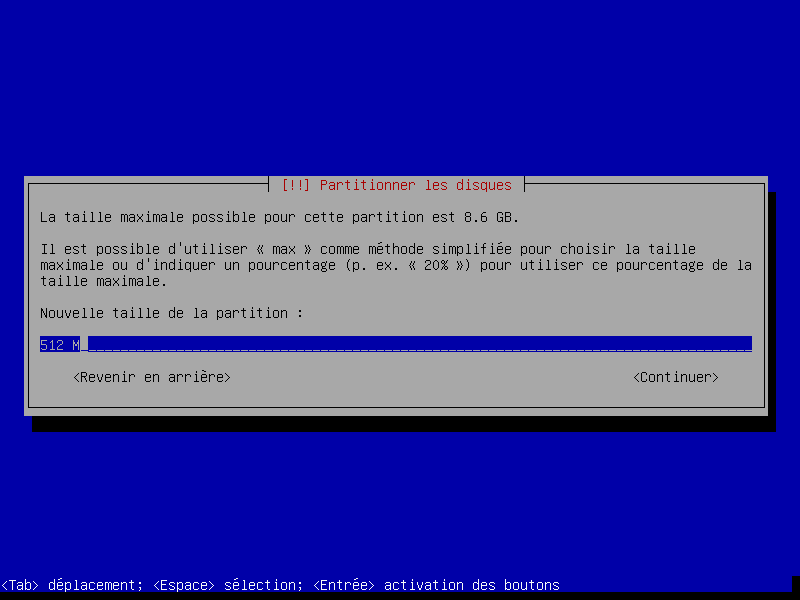
\includegraphics[width=0.7\textwidth]{img/debian7-23.png} } 
& \vspace{0pt} If needed, you'll be able to create some other swap files later, for now, "512 M" is enough. 
\end{longtable}
\end{center}
\begin{center} \newcolumntype{M}[1]{>{\arraybackslash}p{#1}} \begin{longtable}{M{12cm}|M{4cm}}
\belowbaseline[0pt-\heightof{X}]{ 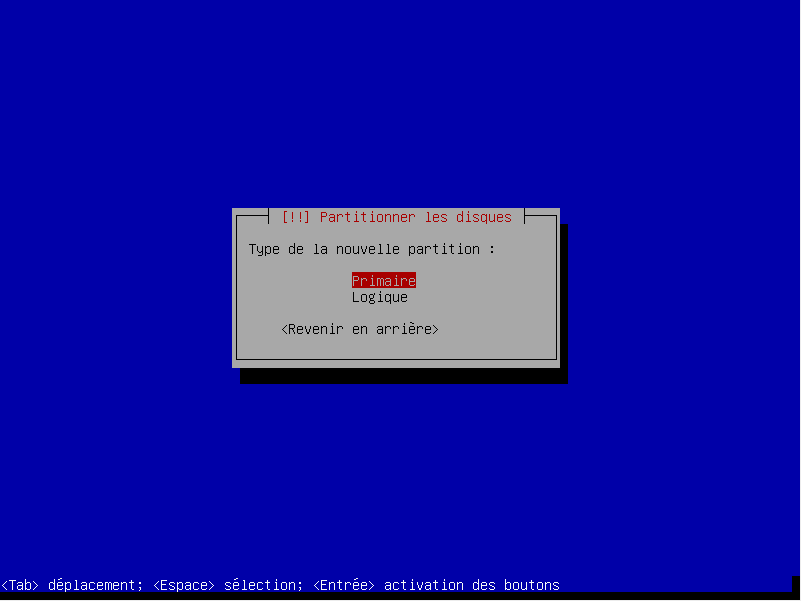
\includegraphics[width=0.7\textwidth]{img/debian7-24.png} } 
& \vspace{0pt} This is a "primary" partition
\end{longtable}
\end{center}
\begin{center} \newcolumntype{M}[1]{>{\arraybackslash}p{#1}} \begin{longtable}{M{12cm}|M{4cm}}
\belowbaseline[0pt-\heightof{X}]{ 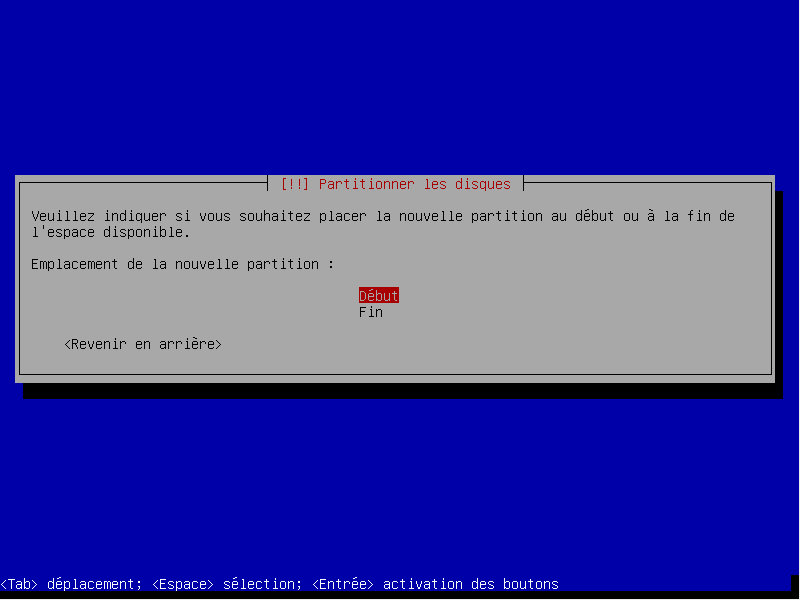
\includegraphics[width=0.7\textwidth]{img/debian7-25.png} } 
& \vspace{0pt} Start this partition in the begining 
\end{longtable}
\end{center}
\begin{center} \newcolumntype{M}[1]{>{\arraybackslash}p{#1}} \begin{longtable}{M{12cm}|M{4cm}}
\belowbaseline[0pt-\heightof{X}]{ 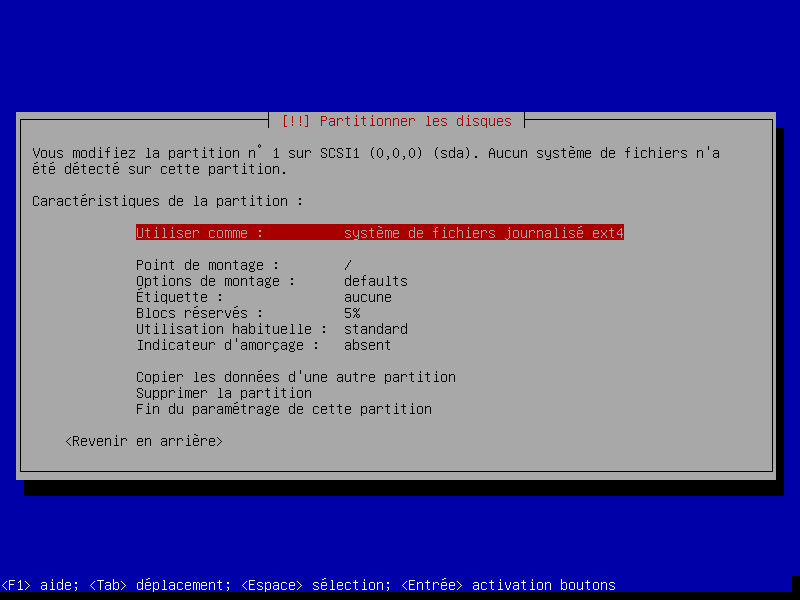
\includegraphics[width=0.7\textwidth]{img/debian7-26.png} } 
& \vspace{0pt} Enter in the "Use as" menu 
\end{longtable}
\end{center}
\begin{center} \newcolumntype{M}[1]{>{\arraybackslash}p{#1}} \begin{longtable}{M{12cm}|M{4cm}}
\belowbaseline[0pt-\heightof{X}]{ 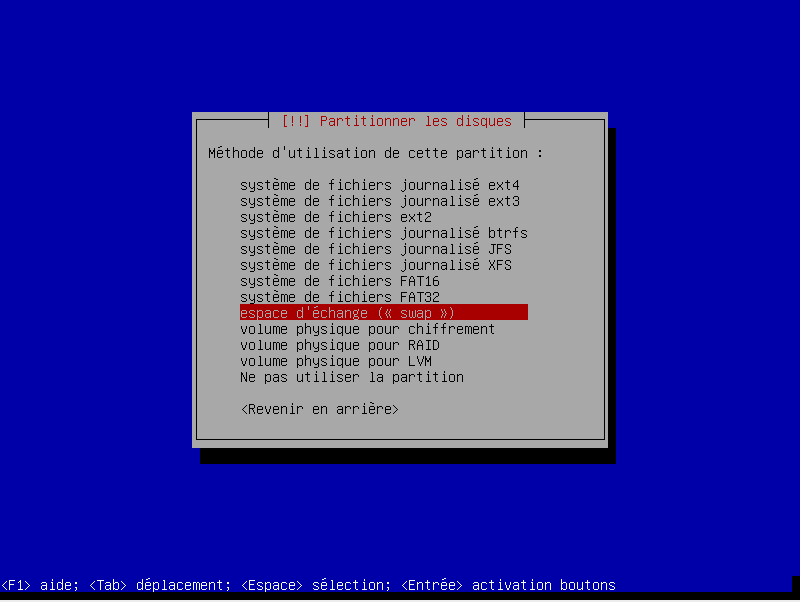
\includegraphics[width=0.7\textwidth]{img/debian7-28.png} } 
& \vspace{0pt} Select SWAP 
\end{longtable}
\end{center}
\begin{center} \newcolumntype{M}[1]{>{\arraybackslash}p{#1}} \begin{longtable}{M{12cm}|M{4cm}}
\belowbaseline[0pt-\heightof{X}]{ 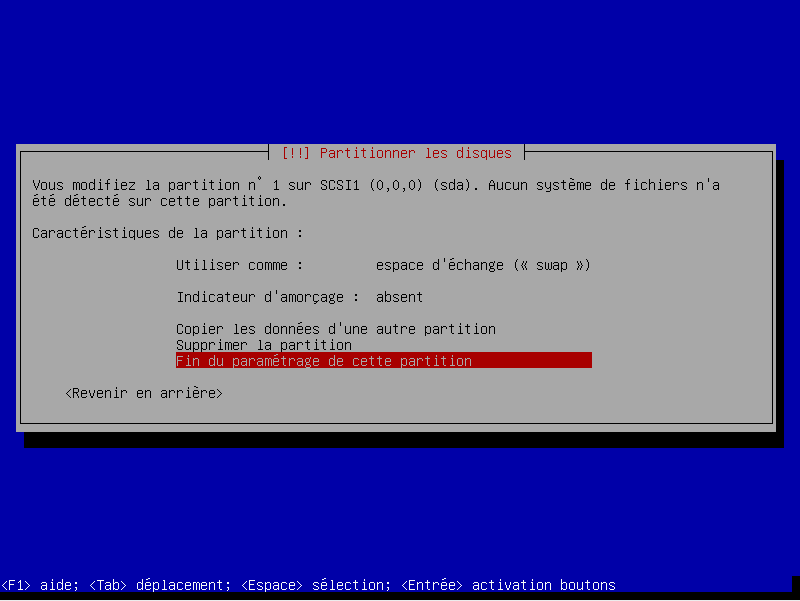
\includegraphics[width=0.7\textwidth]{img/debian7-29.png} } 
& \vspace{0pt} The swap partition configuration is finished 
\end{longtable}
\end{center}
\begin{center} \newcolumntype{M}[1]{>{\arraybackslash}p{#1}} \begin{longtable}{M{12cm}|M{4cm}}
\belowbaseline[0pt-\heightof{X}]{ 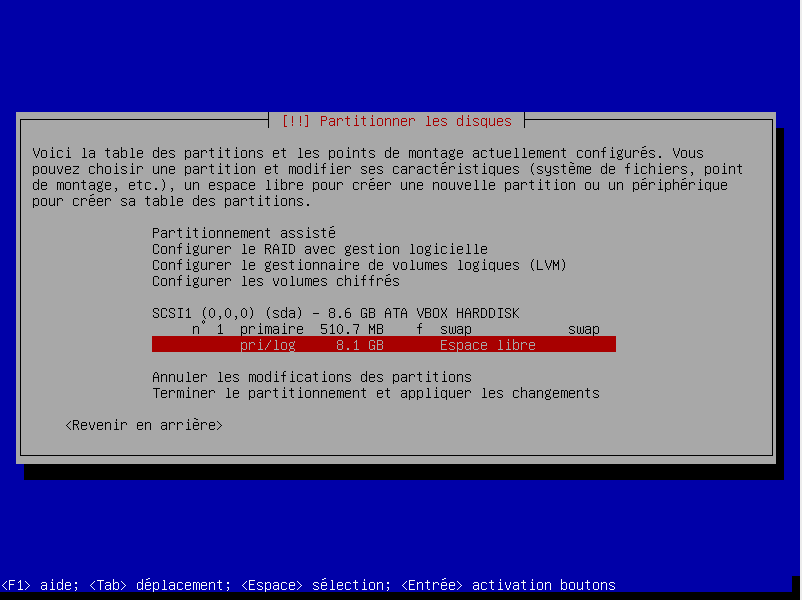
\includegraphics[width=0.7\textwidth]{img/debian7-30.png} } 
& \vspace{0pt} Enter into the empty/free disk space 
\end{longtable}
\end{center}
\begin{center} \newcolumntype{M}[1]{>{\arraybackslash}p{#1}} \begin{longtable}{M{12cm}|M{4cm}}
\belowbaseline[0pt-\heightof{X}]{ 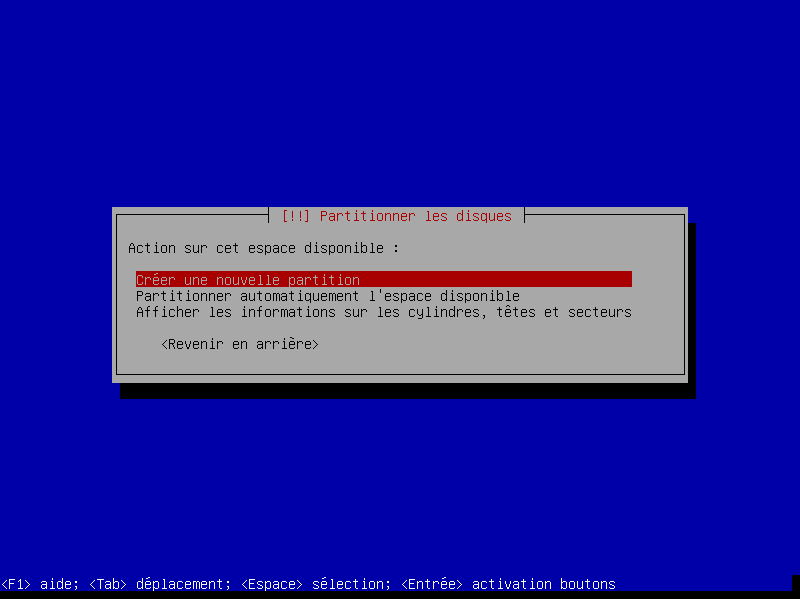
\includegraphics[width=0.7\textwidth]{img/debian7-31.png} } 
& \vspace{0pt} Create a new partition for the main space ( / ) 
\end{longtable}
\end{center}
\begin{center} \newcolumntype{M}[1]{>{\arraybackslash}p{#1}} \begin{longtable}{M{12cm}|M{4cm}}
\belowbaseline[0pt-\heightof{X}]{ 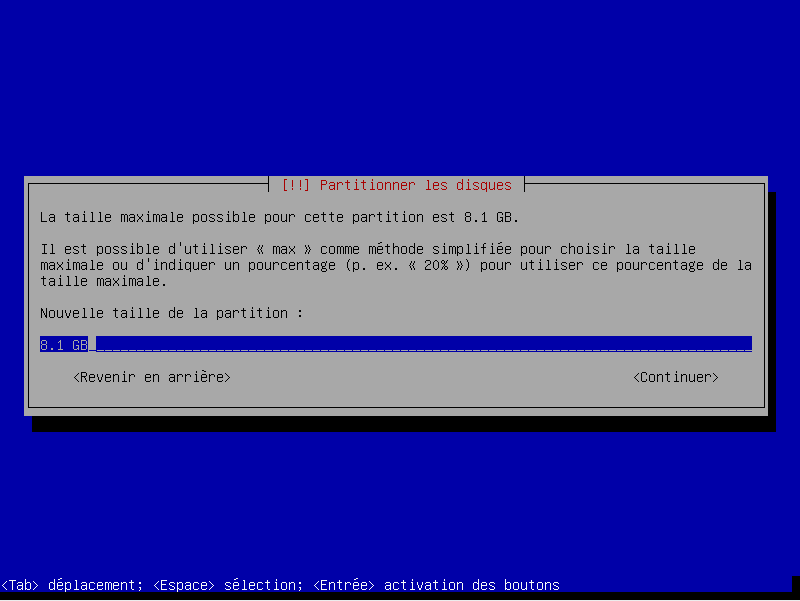
\includegraphics[width=0.7\textwidth]{img/debian7-32.png} } 
& \vspace{0pt} Just click [ENTER] to use all the disk available 
\end{longtable}
\end{center}
\begin{center} \newcolumntype{M}[1]{>{\arraybackslash}p{#1}} \begin{longtable}{M{12cm}|M{4cm}}
\belowbaseline[0pt-\heightof{X}]{ 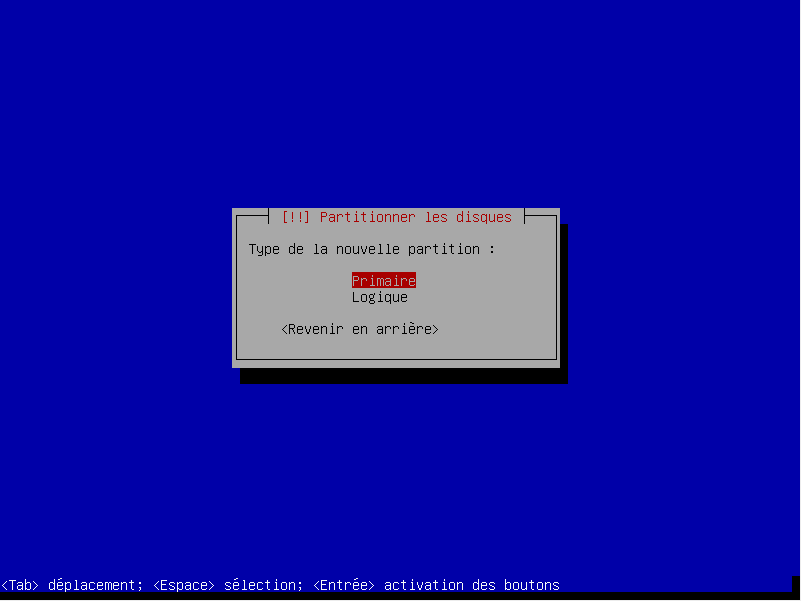
\includegraphics[width=0.7\textwidth]{img/debian7-33.png} } 
& \vspace{0pt} "Primary" partion too 
\end{longtable}
\end{center}
\begin{center} \newcolumntype{M}[1]{>{\arraybackslash}p{#1}} \begin{longtable}{M{12cm}|M{4cm}}
\belowbaseline[0pt-\heightof{X}]{ 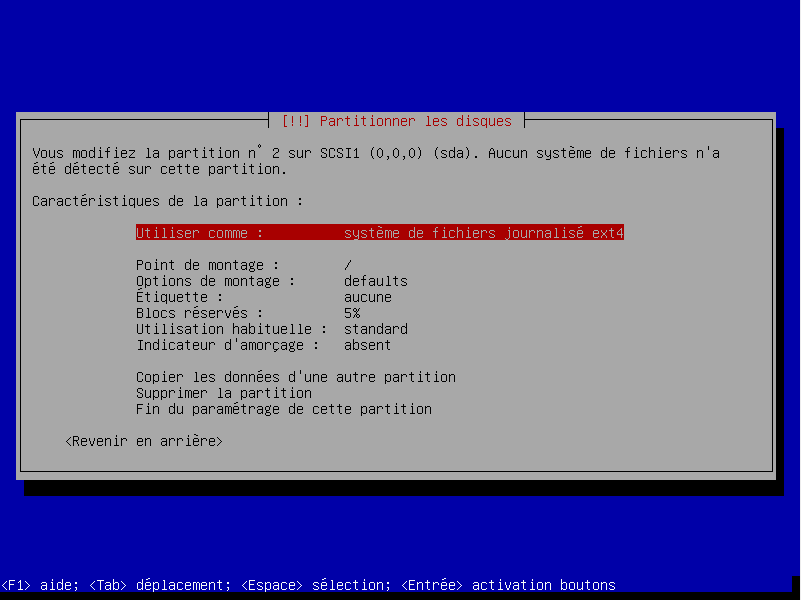
\includegraphics[width=0.7\textwidth]{img/debian7-34.png} } 
& \vspace{0pt} Use "ext4" file system
\end{longtable}
\end{center}
\begin{center} \newcolumntype{M}[1]{>{\arraybackslash}p{#1}} \begin{longtable}{M{12cm}|M{4cm}}
\belowbaseline[0pt-\heightof{X}]{ 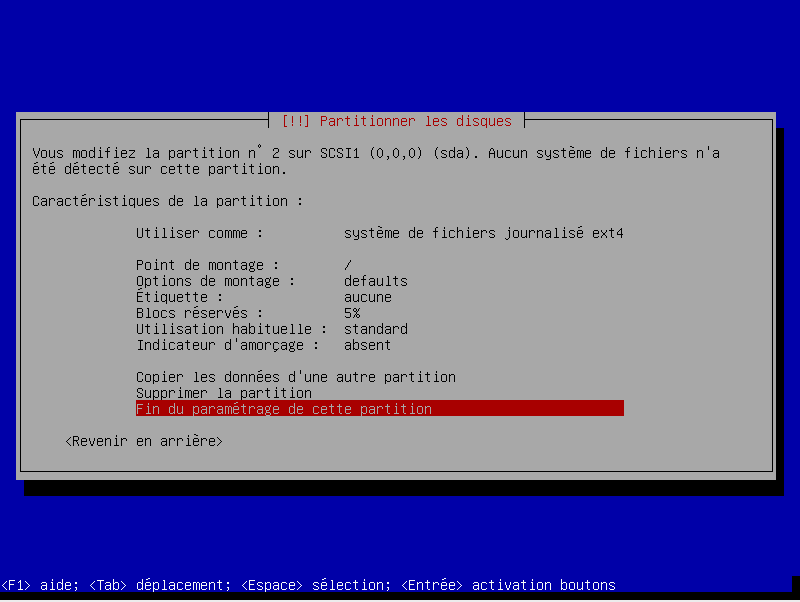
\includegraphics[width=0.7\textwidth]{img/debian7-35.png} } 
& \vspace{0pt} Finish to edit the partition
\end{longtable}
\end{center}
\begin{center} \newcolumntype{M}[1]{>{\arraybackslash}p{#1}} \begin{longtable}{M{12cm}|M{4cm}}
\belowbaseline[0pt-\heightof{X}]{ 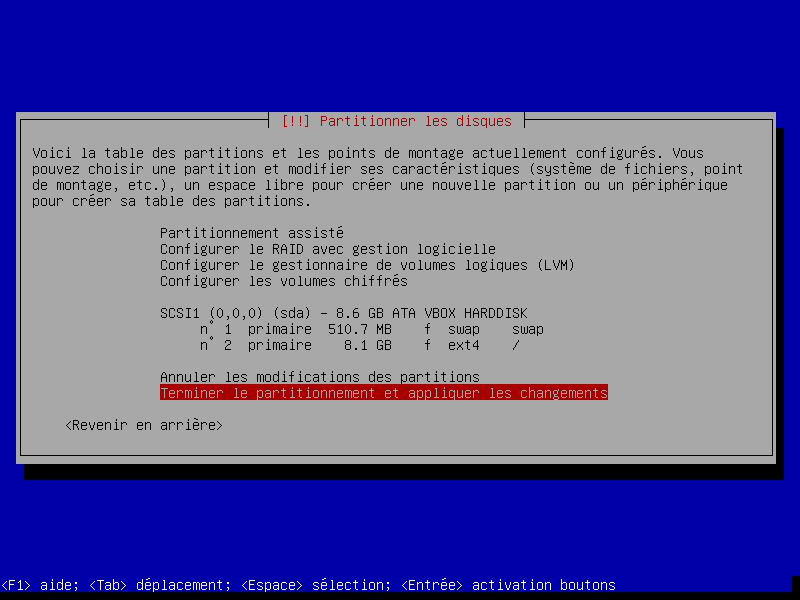
\includegraphics[width=0.7\textwidth]{img/debian7-36.png} } 
& \vspace{0pt} Finish to edit the hard drive partitionning 
\end{longtable}
\end{center}
\begin{center} \newcolumntype{M}[1]{>{\arraybackslash}p{#1}} \begin{longtable}{M{12cm}|M{4cm}}
\belowbaseline[0pt-\heightof{X}]{ 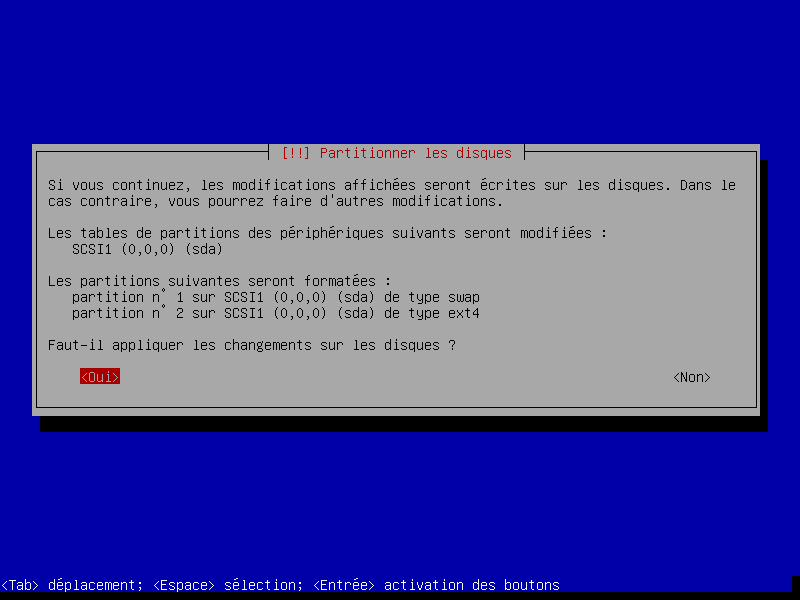
\includegraphics[width=0.7\textwidth]{img/debian7-37.png} } 
& \vspace{0pt} Yes, apply this hard drive configuration 
\end{longtable}
\end{center}

\section{Installer le systeme de base}
\begin{center} \newcolumntype{M}[1]{>{\arraybackslash}p{#1}} \begin{longtable}{M{12cm}|M{4cm}}
\belowbaseline[0pt-\heightof{X}]{ 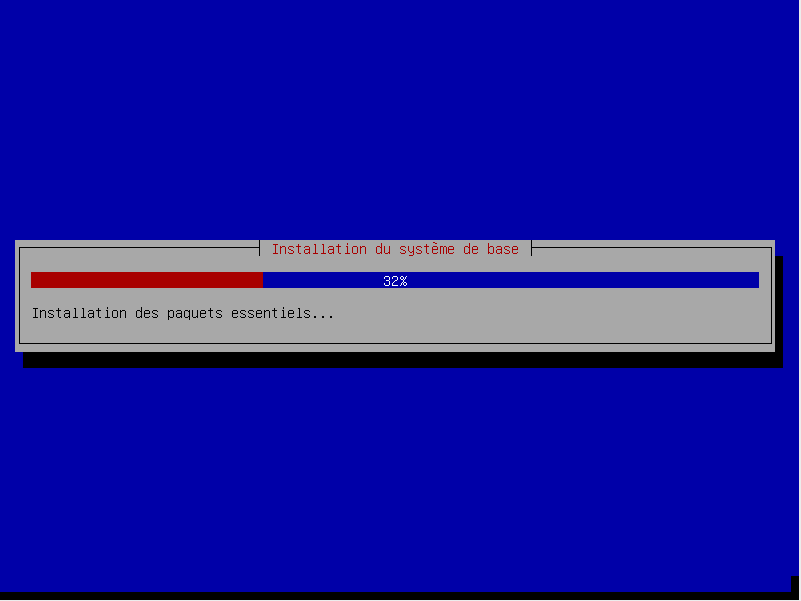
\includegraphics[width=0.7\textwidth]{img/debian7-38.png} } 
& \vspace{0pt} The system is loading the needed packages for the installation 
\end{longtable}
\end{center}

\section{Configurer l'outil de gestion des paquets}
\begin{center} \newcolumntype{M}[1]{>{\arraybackslash}p{#1}} \begin{longtable}{M{12cm}|M{4cm}}
\belowbaseline[0pt-\heightof{X}]{ 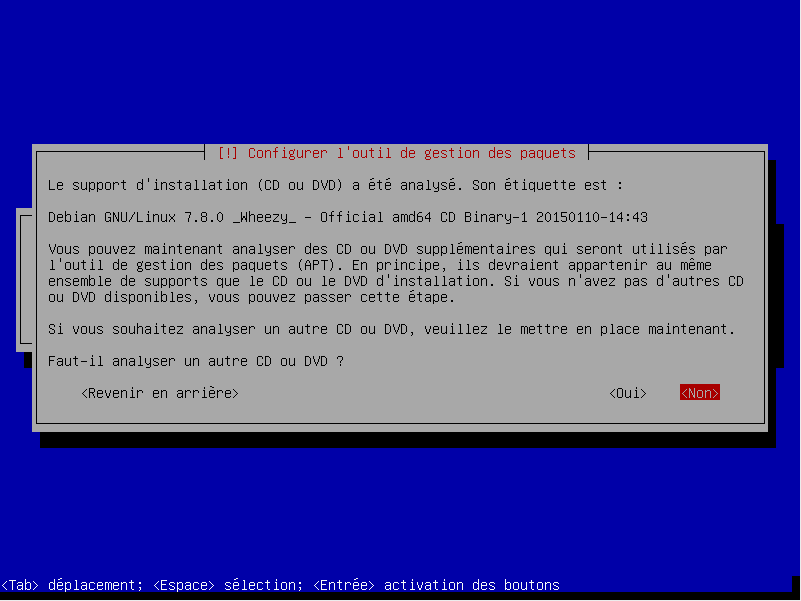
\includegraphics[width=0.7\textwidth]{img/debian7-39.png} } 
& \vspace{0pt} We don't need to use some other Debian's CD
\end{longtable}
\end{center}
\begin{center} \newcolumntype{M}[1]{>{\arraybackslash}p{#1}} \begin{longtable}{M{12cm}|M{4cm}}
\belowbaseline[0pt-\heightof{X}]{ 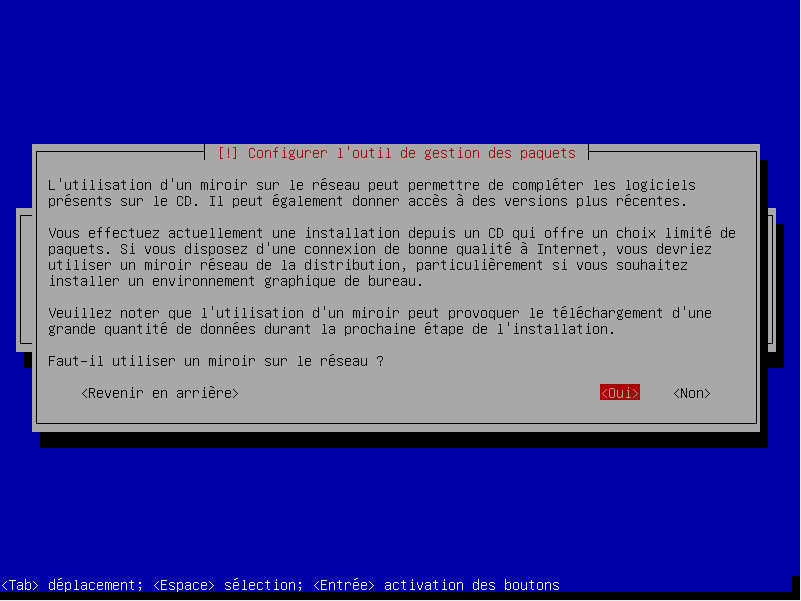
\includegraphics[width=0.7\textwidth]{img/debian7-40.png} } 
& \vspace{0pt} But, "Yes", we'll use a network mirror to be able to download some other packages during the installation
\end{longtable}
\end{center}
\begin{center} \newcolumntype{M}[1]{>{\arraybackslash}p{#1}} \begin{longtable}{M{12cm}|M{4cm}}
\belowbaseline[0pt-\heightof{X}]{ 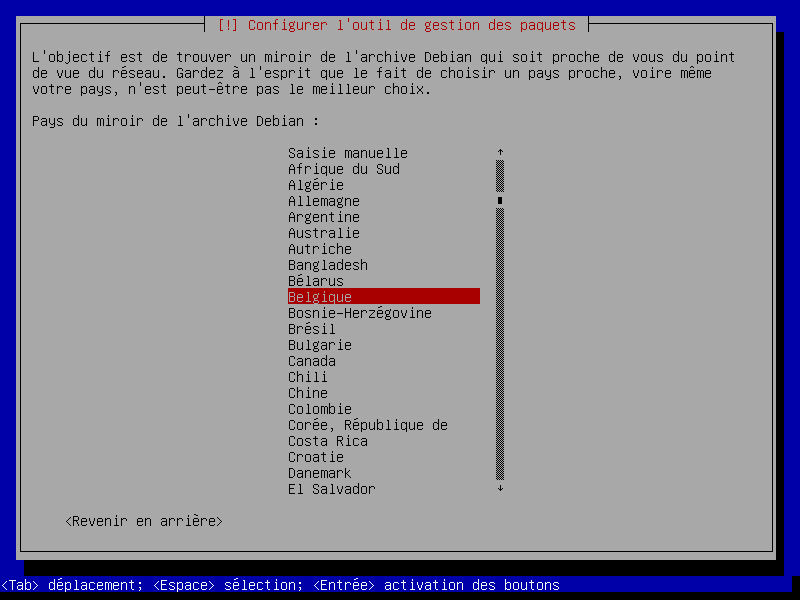
\includegraphics[width=0.7\textwidth]{img/debian7-41.png} } 
& \vspace{0pt} The neerest location will be faster 
\end{longtable}
\end{center}
\begin{center} \newcolumntype{M}[1]{>{\arraybackslash}p{#1}} \begin{longtable}{M{12cm}|M{4cm}}
\belowbaseline[0pt-\heightof{X}]{ 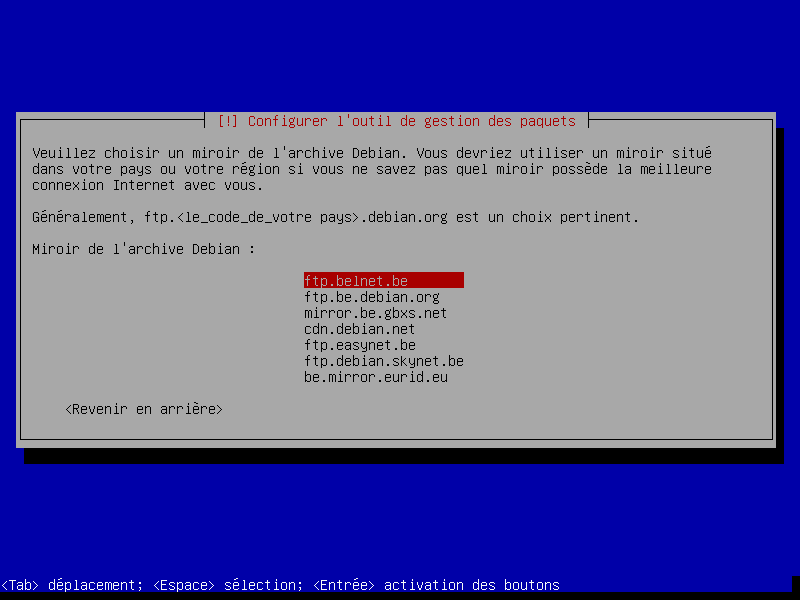
\includegraphics[width=0.7\textwidth]{img/debian7-42.png} } 
& \vspace{0pt} Select a mirror link
\end{longtable}
\end{center}
\begin{center} \newcolumntype{M}[1]{>{\arraybackslash}p{#1}} \begin{longtable}{M{12cm}|M{4cm}}
\belowbaseline[0pt-\heightof{X}]{ 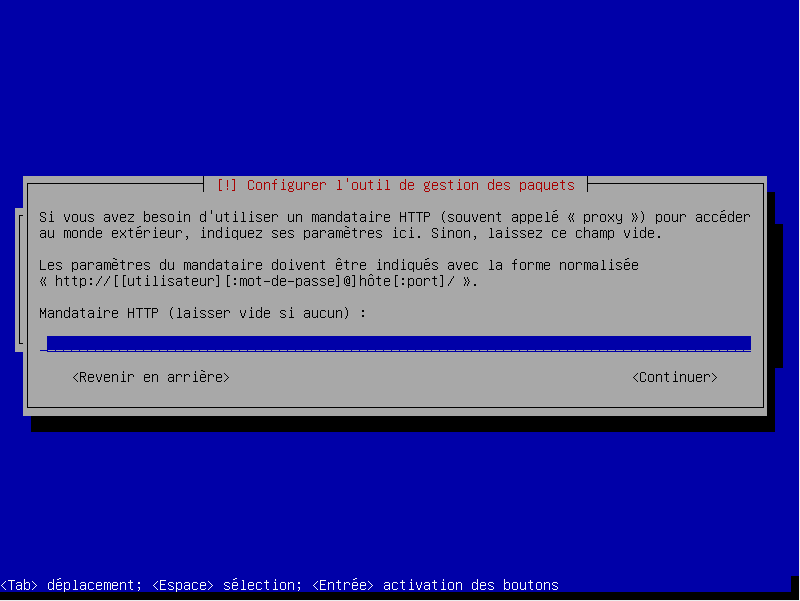
\includegraphics[width=0.7\textwidth]{img/debian7-43.png} } 
& \vspace{0pt} no mandatory http
\end{longtable}
\end{center}
\begin{center} \newcolumntype{M}[1]{>{\arraybackslash}p{#1}} \begin{longtable}{M{12cm}|M{4cm}}
\belowbaseline[0pt-\heightof{X}]{ 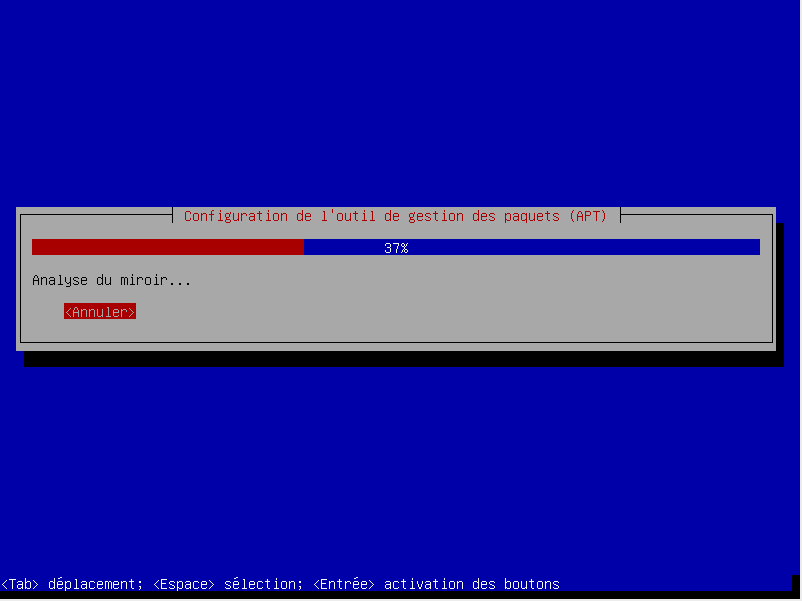
\includegraphics[width=0.7\textwidth]{img/debian7-44.png} } 
& \vspace{0pt} Mirror scanning and update
\end{longtable}
\end{center}

\section{Choisir et installer des logiciels}
\begin{center} \newcolumntype{M}[1]{>{\arraybackslash}p{#1}} \begin{longtable}{M{12cm}|M{4cm}}
\belowbaseline[0pt-\heightof{X}]{ 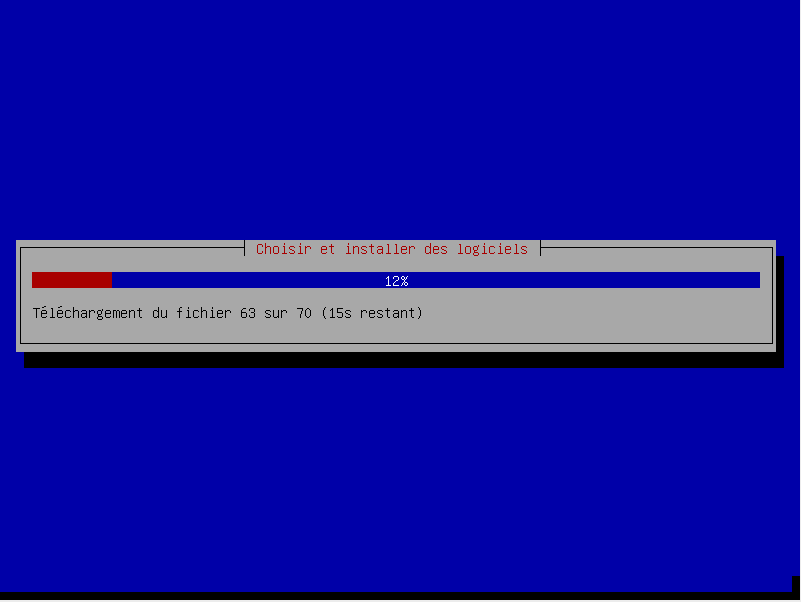
\includegraphics[width=0.7\textwidth]{img/debian7-46.png} } 
& \vspace{0pt} Basic system is loading
\end{longtable}
\end{center}
\begin{center} \newcolumntype{M}[1]{>{\arraybackslash}p{#1}} \begin{longtable}{M{12cm}|M{4cm}}
\belowbaseline[0pt-\heightof{X}]{ 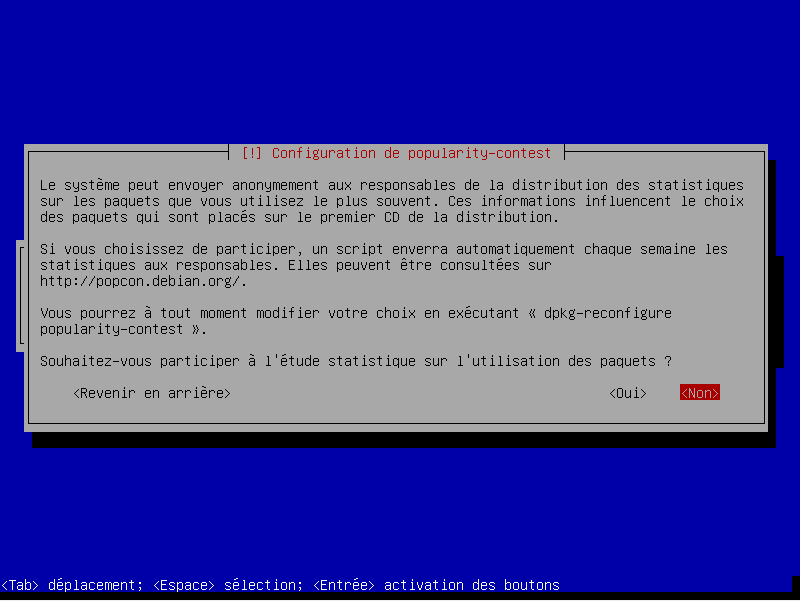
\includegraphics[width=0.7\textwidth]{img/debian7-47.png} } 
& \vspace{0pt} If you want, you can participate to the packages survey
\end{longtable}
\end{center}
\begin{center} \newcolumntype{M}[1]{>{\arraybackslash}p{#1}} \begin{longtable}{M{12cm}|M{4cm}}
\belowbaseline[0pt-\heightof{X}]{ 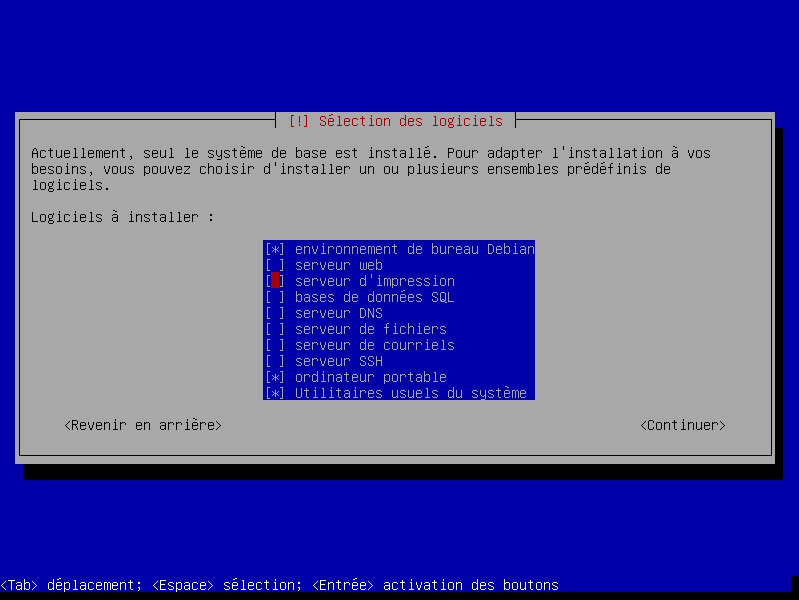
\includegraphics[width=0.7\textwidth]{img/debian7-48.png} } 
& \vspace{0pt} Select global packages: GUI, laptop packages, Base system packages
\end{longtable}
\end{center}
\begin{center} \newcolumntype{M}[1]{>{\arraybackslash}p{#1}} \begin{longtable}{M{12cm}|M{4cm}}
\belowbaseline[0pt-\heightof{X}]{ 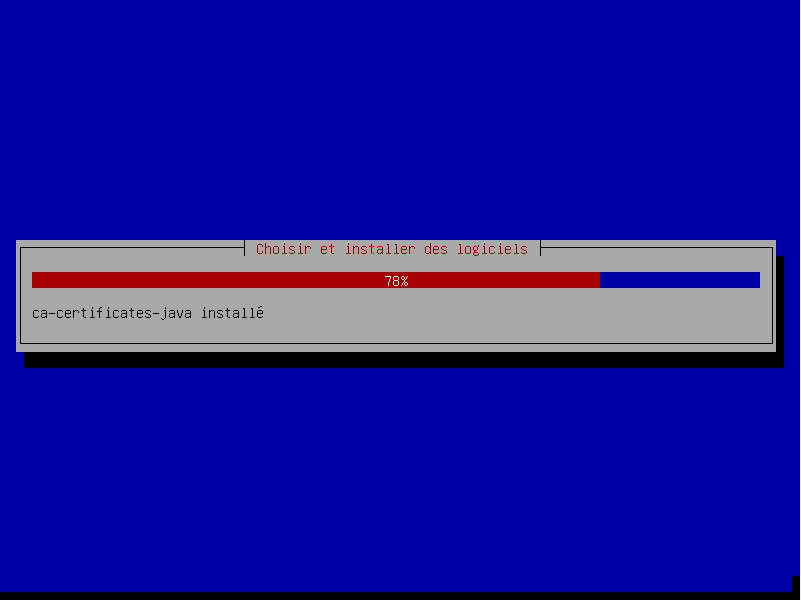
\includegraphics[width=0.7\textwidth]{img/debian7-59.png} } 
& \vspace{0pt} Installing all packages
\end{longtable}
\end{center}

\section{Installer GRUB sur le disque}
\begin{center} \newcolumntype{M}[1]{>{\arraybackslash}p{#1}} \begin{longtable}{M{12cm}|M{4cm}}
\belowbaseline[0pt-\heightof{X}]{ \includegraphics[width=0.7\textwidth]{img/debian7-60.png} } 
& \vspace{0pt} Loading grub packages
\end{longtable}
\end{center}
\begin{center} \newcolumntype{M}[1]{>{\arraybackslash}p{#1}} \begin{longtable}{M{12cm}|M{4cm}}
\belowbaseline[0pt-\heightof{X}]{ \includegraphics[width=0.7\textwidth]{img/debian7-61.png} } 
& \vspace{0pt} "Yes", I want GRUB as default bootloader  
\end{longtable}
\end{center}
\begin{center} \newcolumntype{M}[1]{>{\arraybackslash}p{#1}} \begin{longtable}{M{12cm}|M{4cm}}
\belowbaseline[0pt-\heightof{X}]{ \includegraphics[width=0.7\textwidth]{img/debian7-73.png} } 
& \vspace{0pt} This is grub's interface (after BIOS loading) 
\end{longtable}
\end{center}

\section{Installer LILO sur le disque}
We'll not cover this install in this tutorial

\section{Continuer sans programme de demarrage}
You need a bootloader ! \\
Select it if you really really know what you are doing.

\section{Terminer l'installation}
\begin{center} \newcolumntype{M}[1]{>{\arraybackslash}p{#1}} \begin{longtable}{M{12cm}|M{4cm}}
\belowbaseline[0pt-\heightof{X}]{ \includegraphics[width=0.7\textwidth]{img/debian7-63.png} } 
& \vspace{0pt} Congratitulation ! You've installed you new Debian OS, enter "continue" to restart and use Debian
\end{longtable}
\end{center}
\begin{center} \newcolumntype{M}[1]{>{\arraybackslash}p{#1}} \begin{longtable}{M{12cm}|M{4cm}}
\belowbaseline[0pt-\heightof{X}]{ \includegraphics[width=0.7\textwidth]{img/debian7-74.png} } 
& \vspace{0pt} Select the user and enter his password
\end{longtable}
\end{center}



\chapter{Conclusion}
\section{Final note}
This install is an easy way, you just need to know some stuff about disk management and follow steps.\\
Depends if you use a CD or a DVD, if you downloaded a CD, you had to choose a specific CD containing a specific GUI (Gnome, KDE, XFCE, LXDE, ...). If it's a DVD, differents packages are all there, you need to enter into the tree to select the disired GUI.

Never forget, Google is you friend !

\chapter{TODO next steps}
\section{What can you do now?}
Now you've got an interface, you can enjoy to learn it an use it as it is, or you can try to open a terminal (or CTRL-F1) and follow any tutorial that can help you to learn CLI commands.

The CLI use is, for me, the fastest way to do, execute, make stuff in a Linux environment, keep going to learn and you will know why :).

\chapter{Annexes}
No Annexes for the moment

\section{Bibliography}
\begin{itemize}
  	\item Debian website \\ {\color{blue} http://www.debian.org}
  	\item \LaTeX website \\ {\color{blue} http://www.latex-project.org}
  	\item GitHub website \\ {\color{blue} http://www.github.com}
  	\item Berny's website \\ {\color{blue} http://www.nakalogic.com}
  	\item Bachelor's evenin schoo website \\ {\color{blue} http://www.promsoc.net}
\end{itemize}


\end{document}
